%% Copyright 2007 Ulf Lindgren
%
% This work may be distributed and/or modified under the conditions of the LaTeX
% Project Public License, either version 1.3 of this license or (at your option)
% any later version. The latest version of this license is in
%   http://www.latex-project.org/lppl.txt
% and version 1.3 or later is part of all distributions of LaTeX version
% 2005/12/01 or later.
%
% This work has the LPPL maintenance status `maintained'.
% 
% The Current Maintainer of this work is Ulf Lindgren.
%
% This work consists of all files listed in manifest.txt.
%
%% This statement added 2010/12/10 by Clea F. Rees following correspondence
%% between Ulf Lindgren and Karl Berry concerning licensing.

\documentclass{report}

 \setlength{\textheight}{23 cm}
 \setlength{\voffset}{-0.54cm}
 \setlength{\hoffset}{-0.54cm}
 \setlength{\oddsidemargin}{0.5 cm}
 \setlength{\evensidemargin}{0.5 cm}
 \setlength{\textwidth}{16 cm}
 \setlength{\marginparwidth}{2.5 cm}
 \setlength{\topmargin}{0.5 cm}
 \setlength{\headheight}{0.5 cm}
 \setlength{\headsep}{0.5 cm}

% \setlength{\voffset}{-5cm}
 \usepackage[T1]{fontenc}
  \usepackage{graphicx}
  \usepackage[Lenny]{fncychap}
  \usepackage{lettrine}
  \newcommand{\sk}{\vspace{0.2 cm}}
  \newcommand{\A}[1]{{$\backslash${\tt #1}}}
  \newcommand{\nsp}{\mbox{\hspace{-1 cm}}}
  \title{FncyChap V1.34}
  \author{Ulf A. Lindgren}
  \date{}
  
\begin{document}
  \maketitle
  \tableofcontents
  \chapter{Package description}
    \lettrine{T}{he package} \textsl{fncychap} has been written such that
    chapter level headings can be altered fast and for me to learn more
    about \LaTeX{} and \TeX{}. I have no idea if this package is
    written in a good way. Thus, if anyone reads and tries {\em
    FncyChap} I would appreciate any feedback. This will help me gain
  insight in writing macros. 
    
    In any publication it is important to remember that consistency
    plays an important role. That is, with this package one can change
    the appearance of each chapter in the publication. However, this is
    not desirable so don't forget modesty and consistency.

    \section{Basic use and requirements}
    The package is invoked by writing the following in the preamble of
    your document\sk\\
    \nsp\fbox{\A{usepackage}[{\em style}]\{{\em fncychap}\}}\sk\\
    If the option, {\em style}, is omitted then the default definition
    of chapter is used. Originally, there were six predefined chapter styles,
    namely {\em Sonny, Lenny, Glenn, Conny, Rejne} and {\em Bjarne}.
    The names corresponds to Swedish given names, almost surely (a.s.)
    like
    IKEA\footnote{reg. trademark of Ingvar Kamprad Emtaryd
    Agunnaryd}. Each such style has a default configuration and if
    that configuration is sufficient, then this is all that is needed.
    
    In the present release of \textsl{fncychap} two additional chapter
    definitions have been included. The first of these is named {\em
      PetersLenny}, after the author Peter Osborn. This chapter
    definition is based on {\em Lenny}, Peter has carefully tweaked
    the measures of the lines, individually, for each chapter number (up to 20)
    and each appendix (up to Z). The second chapter head is a new one
    defined by Jean-Marc Francois and he named it \textsl{Bjornstrup}.

    Originally, \textsl{fncychap} did not rely on any other package. However, for the
    style {\tt Lenny} a postscript font is default, but this font can
    easily be changed. I encourage the use of the default postscript
    font since it is scalable in a truly huge manner, which makes
    {\em Lenny} nice. In the current release and with the use of
    Jean-Marcs \textsl{Bjornstrup} the color package from the base
    distribution will be invoked.
    
  \chapter{Commands provided}
  \lettrine{A}{part from the chapter styles}, some additional commands are
  provided in order to create user defined chapter heads. The commands
  will in the sequel be described. Each command is boxed and placed on
  a separate line. Lets begin the descriptions of the commands.\sk\\ 
  \nsp\fbox{\A{mghrulefill}\{{\em width}\}}\sk\\
  The above command is a more general version of the command
  \A{hrulefill} in the sense that the width of the ruler can be
  specified. This command is provided in order to decorate the chapter
  headers. The chapter heading are divided into two parts. The first
  part defines the so called \A{chapapp} and \A{thechapter} which
  holds information of the text ``Chapter'' and the current chapter number
  respectively. The second part is the chapter title provided by the
  user. From now one, the \A{chapapp} and \A{thechapter} will be
  referred to as chapter name and chapter number respectively. The
  user defined title is referred to as the chapter title.

  \section{Toward customization of the chapter head}
  \label{sec:TW}
    The chapter name, number and title can be changed easy, first lets
    introduce the following two commands\sk\\
    \nsp\fbox{\A{ChNameUpperCase}}\sk\\
    and\sk\\
    \nsp\fbox{\A{ChNameLowerCase}}\sk\\
    these commands will change the chapter name into either upper or
    lower case. One additional case command is provided for the
    chapter name, namely\sk\\
    \nsp\fbox{\A{ChNameAsIs}}\sk\\
    which result in the default case. Three similar commands for the
    chapter title are defined by the commands\sk\\
    \nsp\fbox{\A{ChTitleUpperCase}, \A{ChTitleLowerCase} and
      \A{ChNameAsIs}}\sk\\
    The rule width of the predefined chapter styles can be controlled
    by the command\sk\\
    \nsp\fbox{\A{ChRuleWidth}\{{\em width}\}}\sk\\
    just remember that the {\em width} must have a unit, for instance
    {\em pt, mm, etc}. The font related matters such as size, type and
    face can be sent using the commands\sk\\
    \nsp\fbox{\A{ChNameVar}\{{\em stuff}\}, \A{ChNumVar}\{{\em stuff}\} and
      \A{ChTitleVar}\{{\em stuff}\}}\sk\\
    related to the chapter name number and title respectively.
    The argument, {\em stuff}, to these functions can be for example
    \mbox{\A{ChNameVar}\{\A{huge}\A{rmfamily}\A{centering}\}}.
    \enlargethispage{1cm}
  \chapter{An overview of the chapter styles}
    \lettrine{T}{he chapter styles} have default settings for all of the functions
    described in section~\ref{sec:TW}. However, it can be changed
    using the commands. Note that if \A{centering}, etc is used to
    format the text part of the chapter style then the result can be
    ugly. The chapter style {\em Bjarne} contains one additional
    command\sk\\
    \nsp\fbox{\A{TheAlphaChapter}}\sk\\
    This command will write the chapter number using the corresponding
    word. \A{TheAlphaChapter} have a capability of writing the words
    {\em ZERO} to {NINETYNINE}.
    

    In the following sections the pre-defined styles are shown along
    with the default settings. Both the \A{chapter} and \A{chapter*}
    are given.
    \section{The chapter Sonny}
    The following settings have been used as default parameters
    {\small\begin{verbatim}  
      \ChNameVar{\Large\sffamily} \ChTitleVar{\Large\sffamily}
      \ChNumVar{\Huge} \ChRuleWidth{0.5pt} \ChNameUpperCase
    \end{verbatim}}    
    \begin{figure}[h]
      \begin{minipage}{7 cm}
        \label{fig:Sonnys}
        \centerline{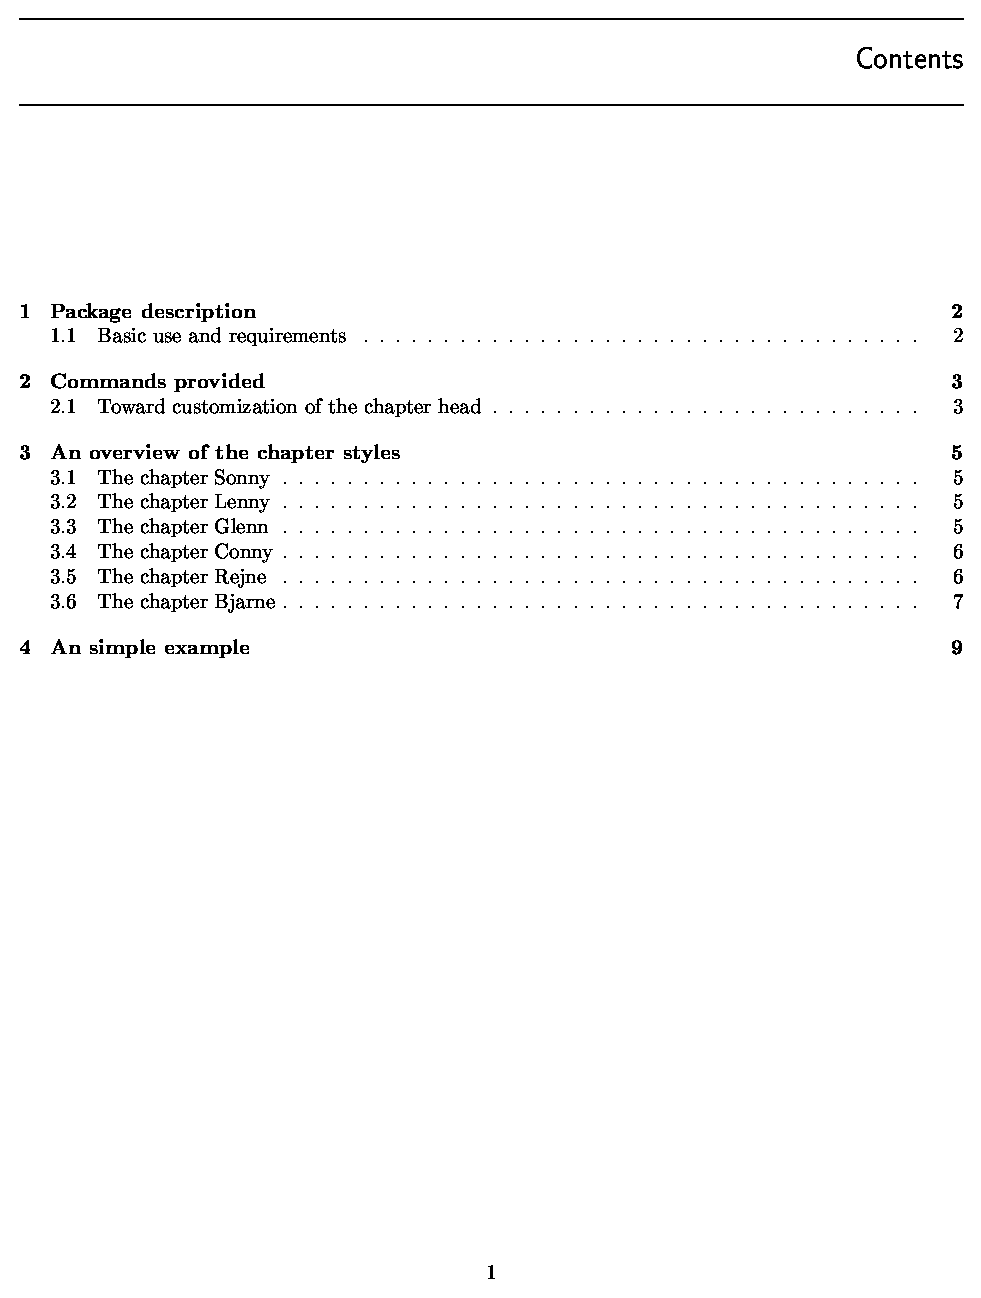
\includegraphics[height=6cm]{Sonnys.eps}} 
        \caption{The stared chapter style sonny}
      \end{minipage}\hfill
      \begin{minipage}{7 cm}
        \label{fig:Sonny}
        \centerline{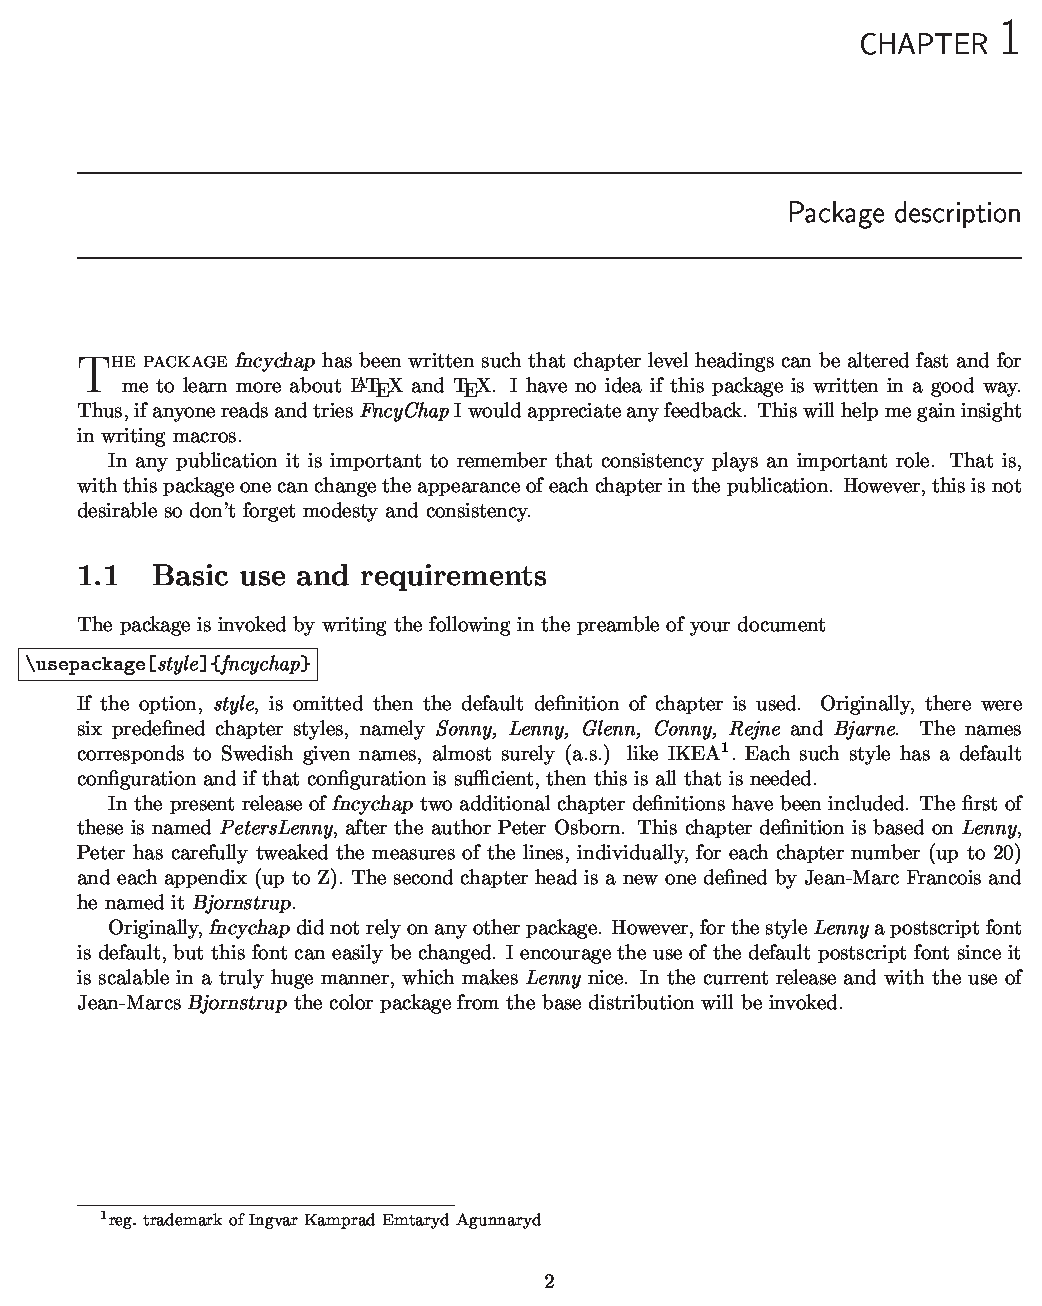
\includegraphics[height=6cm]{Sonny.eps}}
        \caption{The chapter style Sonny}
      \end{minipage}\hfill
    \end{figure}    
    
% \clearpage
    \section{The chapter Lenny}
    The following settings have been used as default parameters
    {\small\begin{verbatim}
      \ChNameVar{\fontsize{14}{16}\usefont{OT1}{phv}{m}{n}\selectfont}
      \ChNumVar{\fontsize{60}{62}\usefont{OT1}{ptm}{m}{n}\selectfont}
      \ChTitleVar{\Huge\bfseries\rmfamily} \ChRuleWidth{1pt}
    \end{verbatim}}
    \begin{figure}[h]
      \begin{minipage}{7 cm}
        \centerline{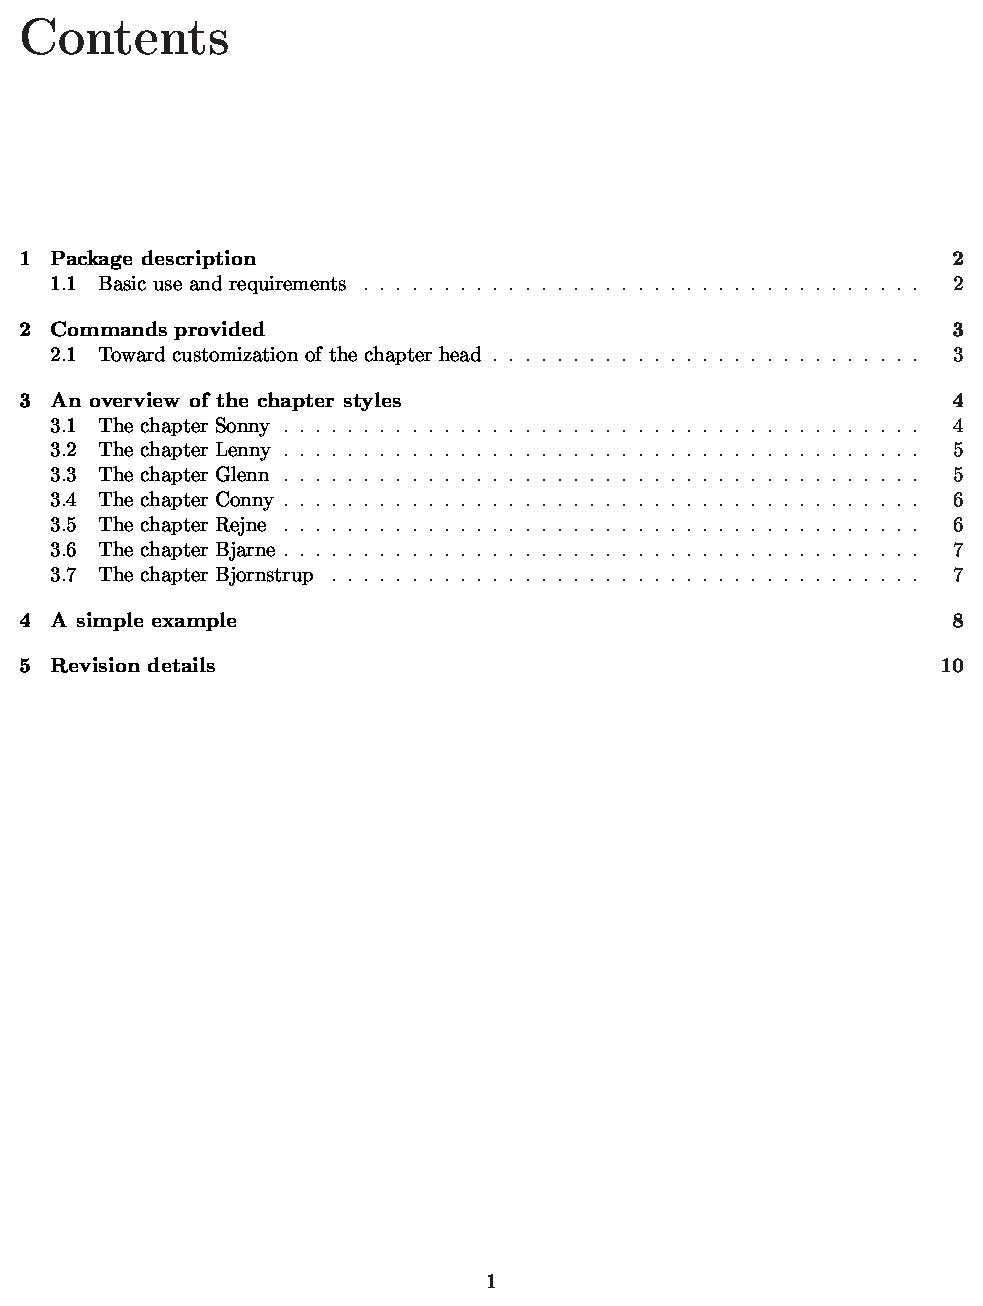
\includegraphics[height=6cm]{Lennys.eps}} 
        \caption{The stared chapter style Lenny}
      \end{minipage}\hfill
      \begin{minipage}{7 cm}
        \centerline{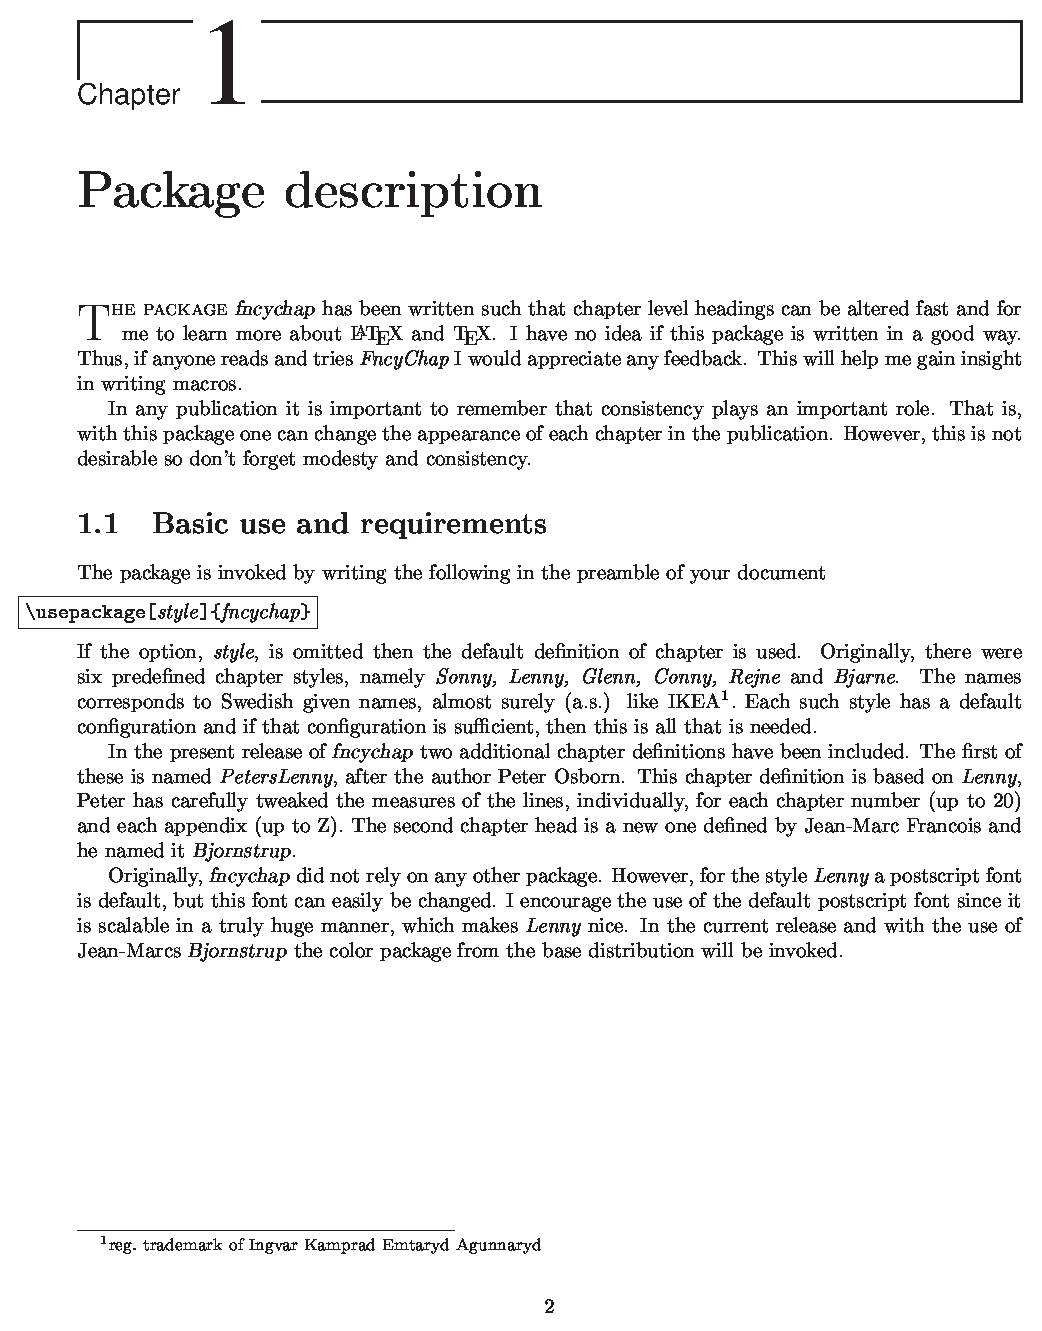
\includegraphics[height=6cm]{Lenny.eps}}
        \caption{The chapter style Lenny}
      \end{minipage}\hfill
    \end{figure}
\textbf{Note:} An alternative version of this chapter head exist
entitled \textsl{PetersLenny}.
%\enlargethispage{2cm}

    \section{The chapter Glenn}
    The following settings have been used as default parameters
    {\small\begin{verbatim}
      \ChNameVar{\bfseries\Large\sffamily} \ChNameUpperCase
      \ChTitleVar{\bfseries\Large\rmfamily} \ChTitleUpperCase
      \ChNumVar{\Huge} \ChRuleWidth{1pt}
    \end{verbatim}}
    \begin{figure}[h]
      \begin{minipage}{7 cm}
        \centerline{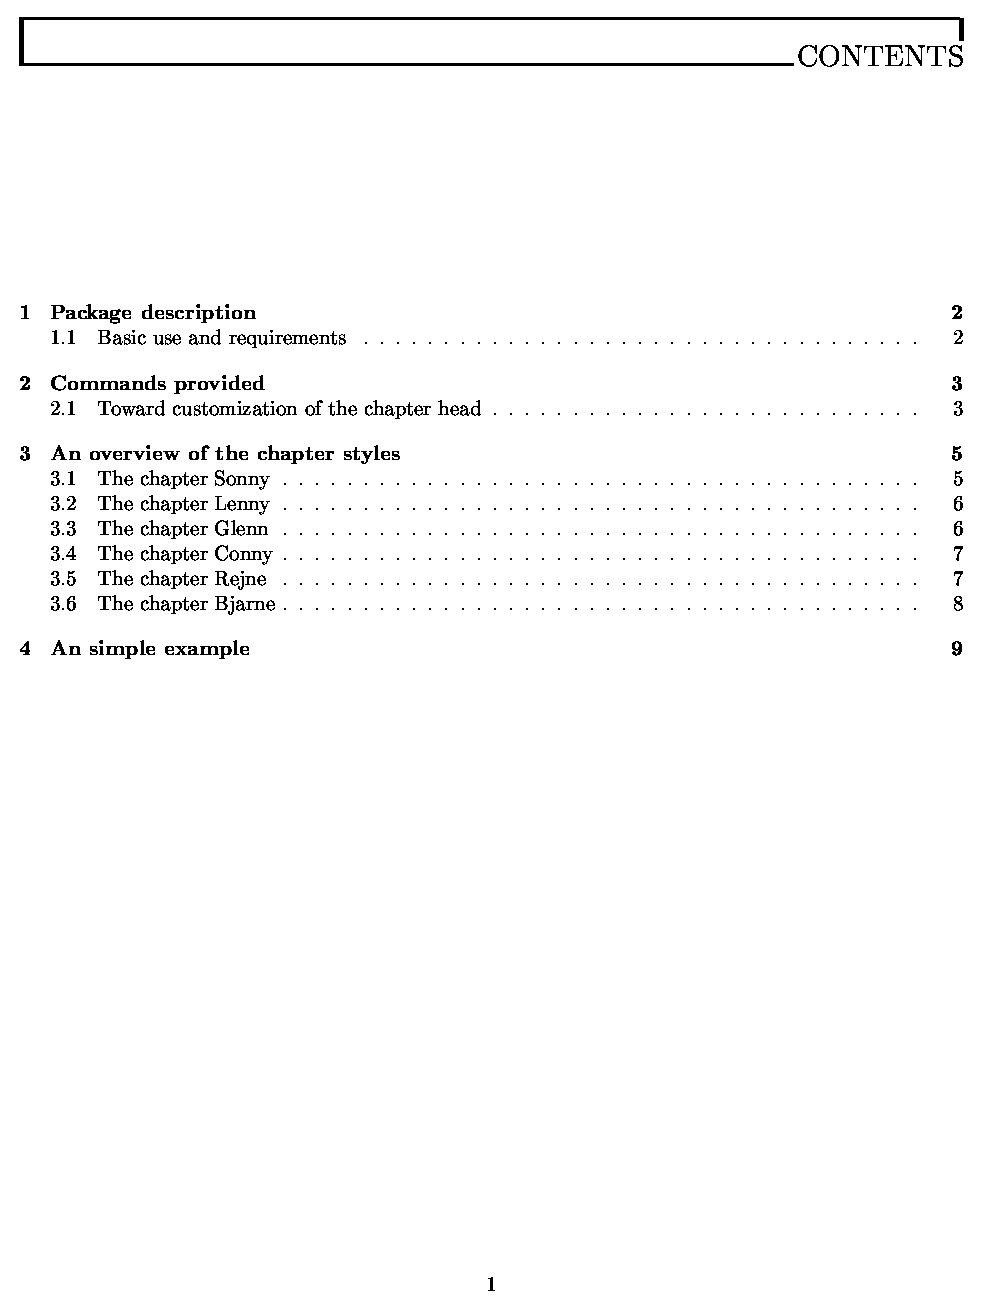
\includegraphics[height=6cm]{Glenns.eps}}
        \caption{The stared chapter style Glenn}
      \end{minipage}\hfill
      \begin{minipage}{7 cm}
        \centerline{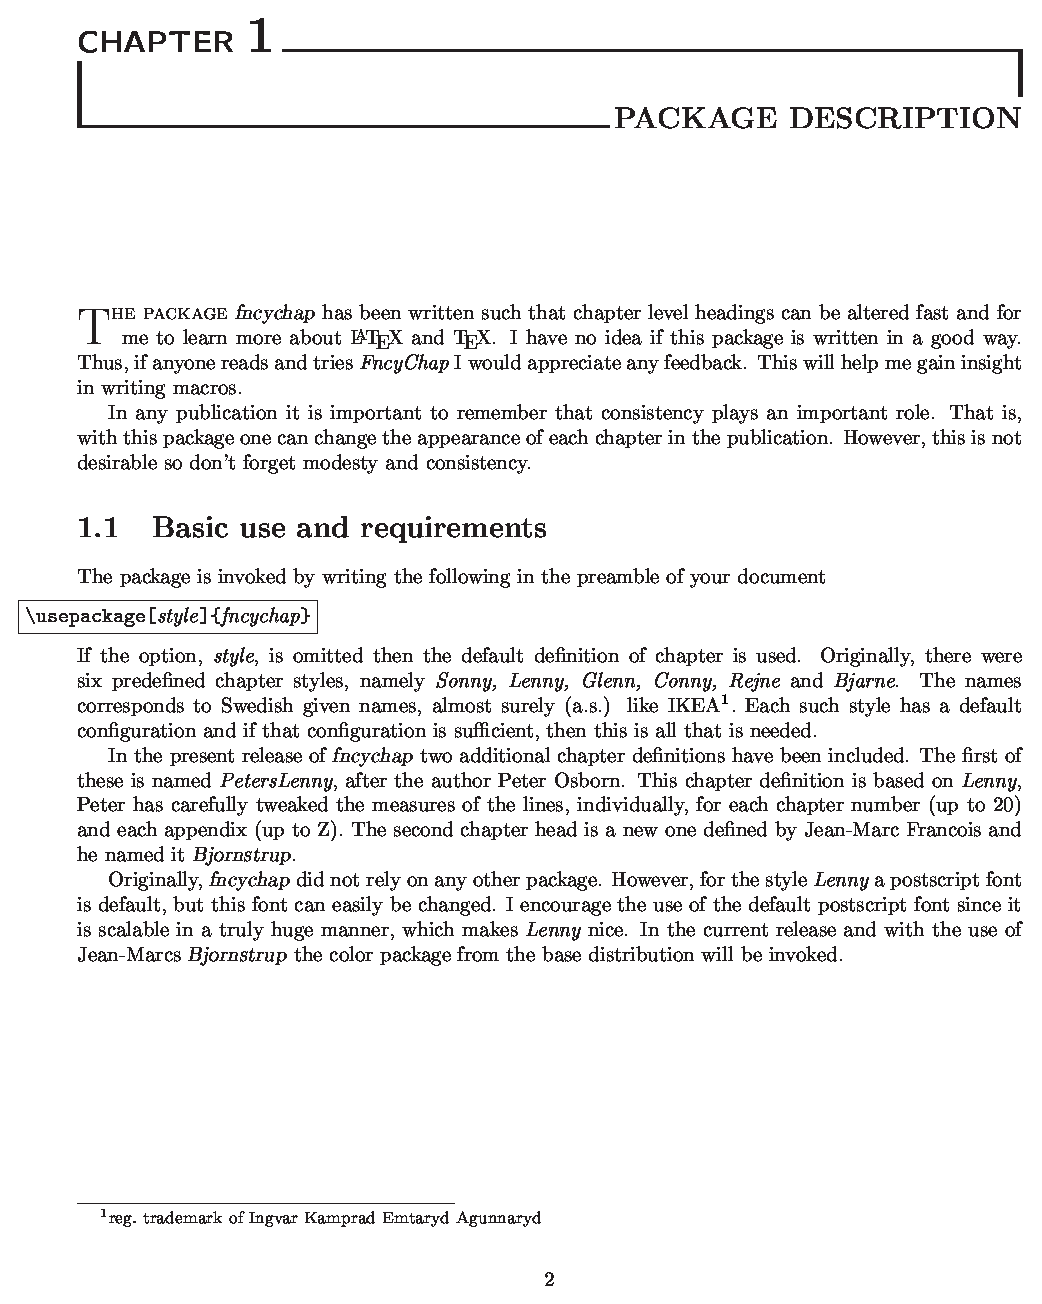
\includegraphics[height=6cm]{Glenn.eps}}
        \caption{The chapter style Glenn}
      \end{minipage}\hfill
    \end{figure}

    \section{The chapter Conny}
    The following settings have been used as default parameters
    {\small\begin{verbatim}
       \ChNameUpperCase \ChNameVar{\centering\Huge\rmfamily\bfseries}
       \ChTitleUpperCase \ChTitleVar{\centering\Huge\rmfamily}
       \ChNumVar{\Huge} \ChRuleWidth{2pt}
    \end{verbatim}}
    \begin{figure}[h]
      \begin{minipage}{7 cm}
        \centerline{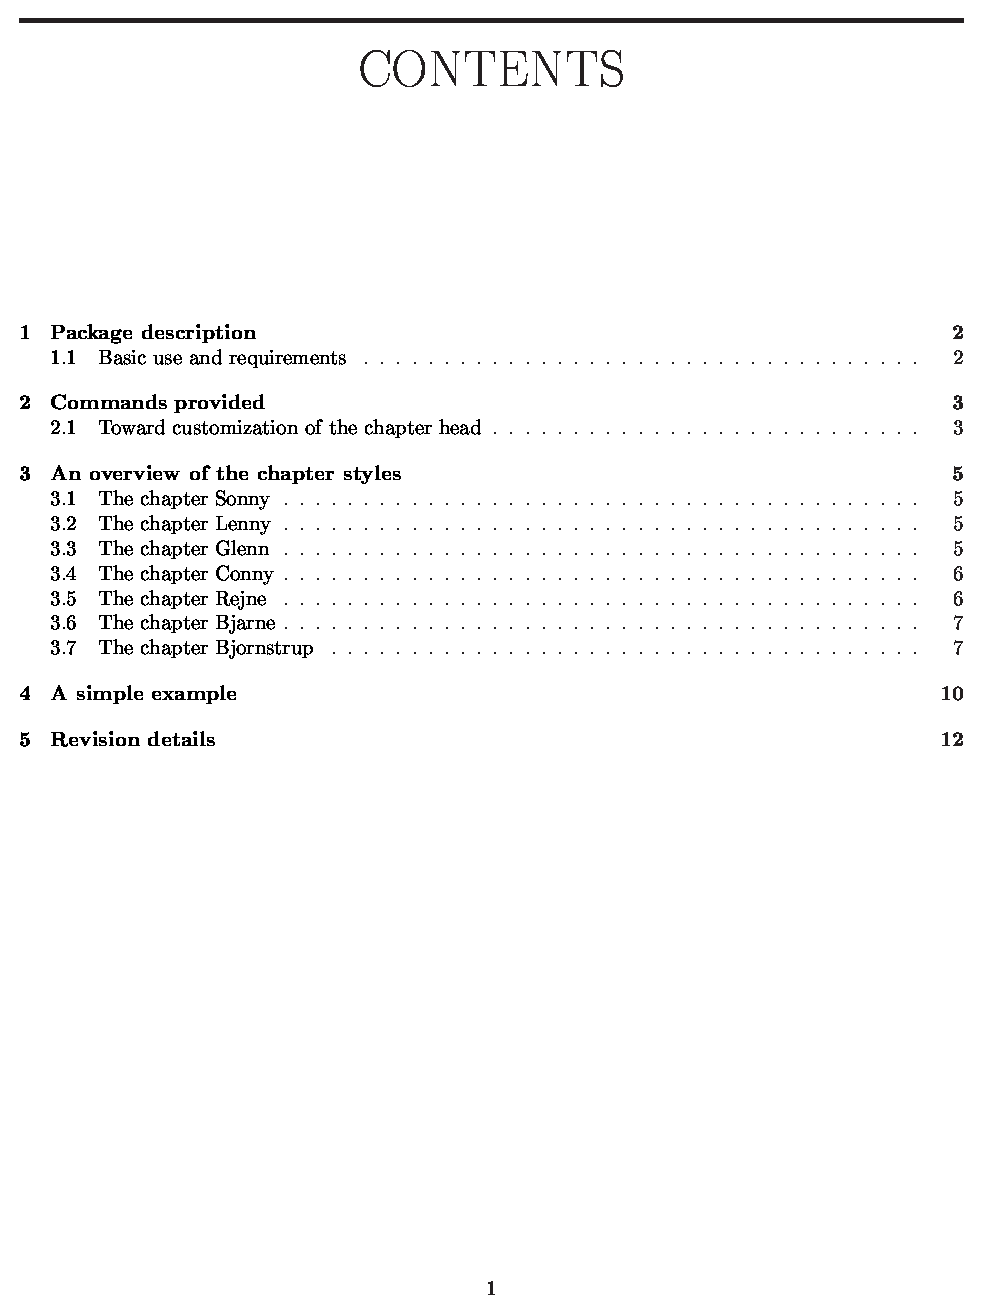
\includegraphics[height=6cm]{Connys.eps}}
        \caption{The stared chapter style Conny}
      \end{minipage}\hfill
      \begin{minipage}{7 cm}
        \centerline{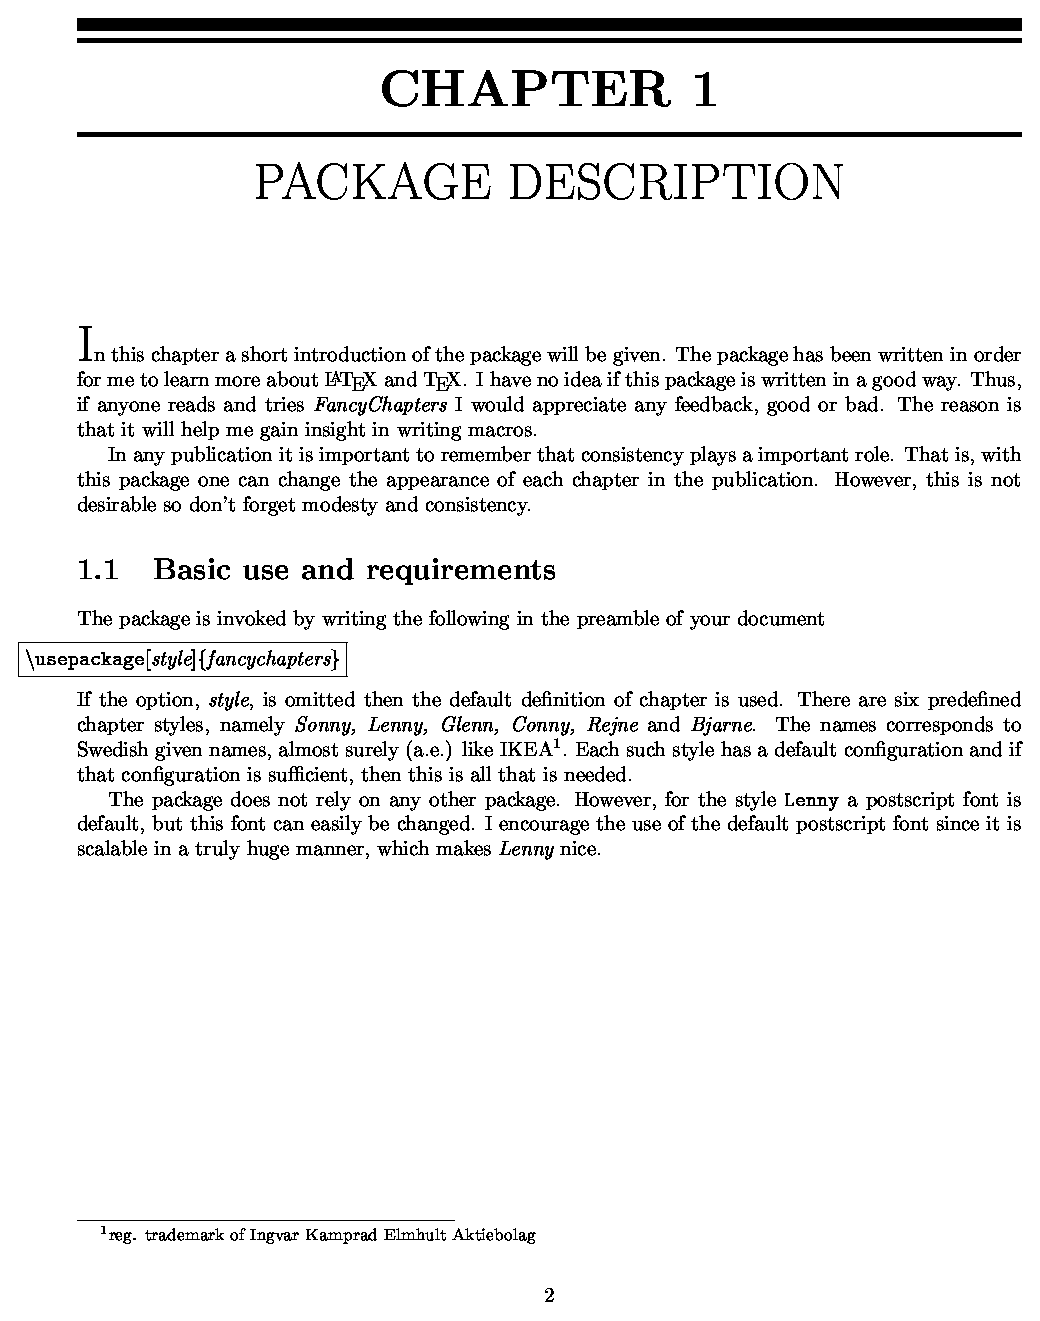
\includegraphics[height=6cm]{Conny.eps}}
        \caption{The chapter style Conny}
      \end{minipage}\hfill
    \end{figure}

    \section{The chapter Rejne}
    The following settings have been used as default parameters
    {\small\begin{verbatim}  
      \ChNameUpperCase \ChNameVar{\centering\Huge\rmfamily\bfseries}
      \ChTitleUpperCase \ChTitleVar{\centering\Huge\rmfamily}
      \ChNumVar{\Huge} \ChRuleWidth{1pt}
   \end{verbatim}}
    \begin{figure}[h]
      \begin{minipage}{7 cm}
        \centerline{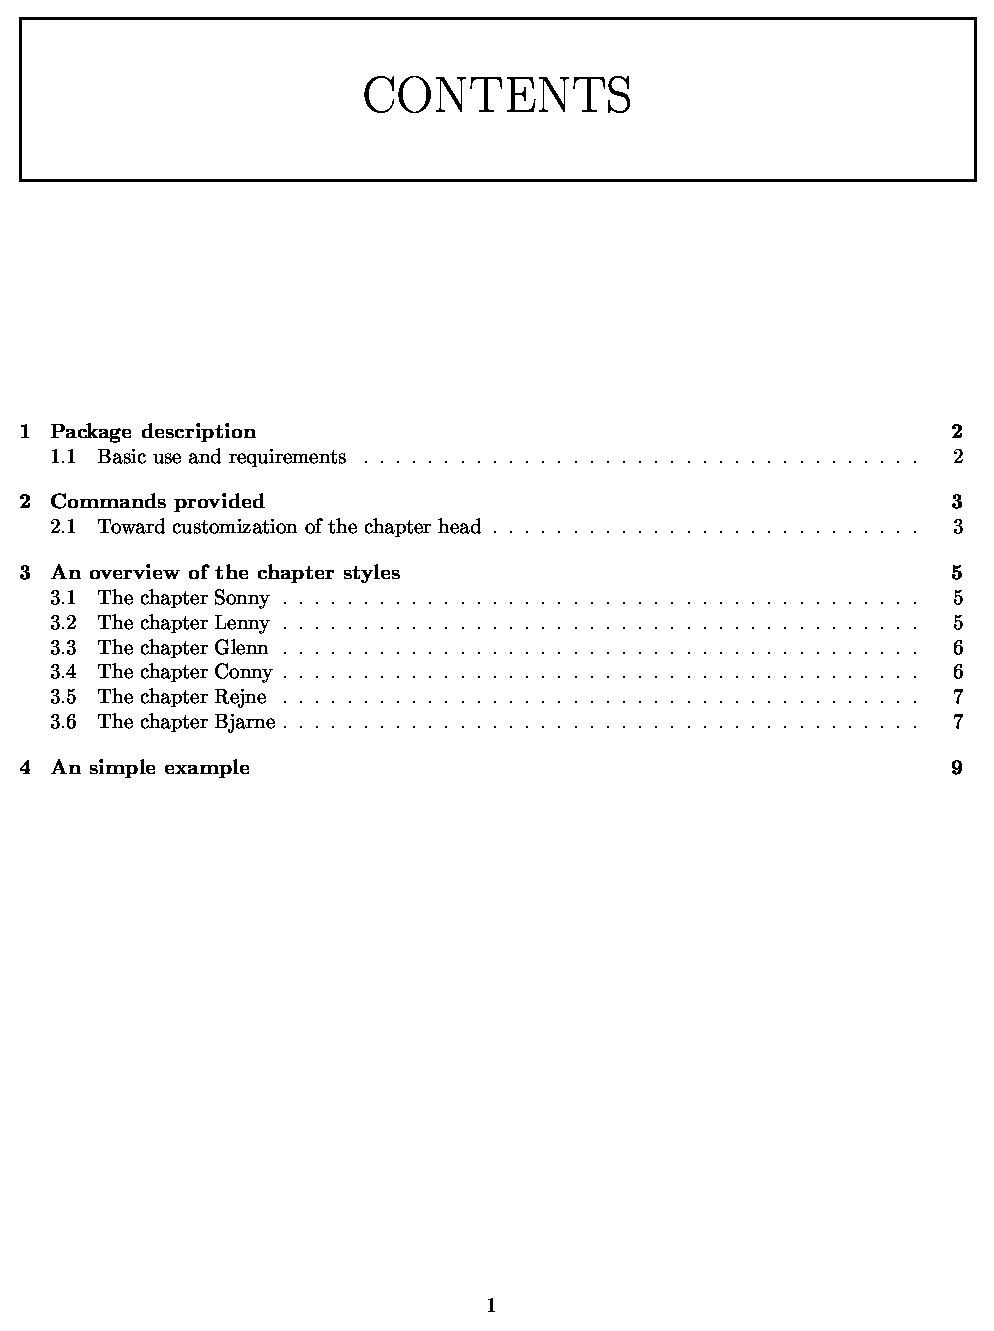
\includegraphics[height=6cm]{Rejnes.eps}}
        \caption{The stared chapter style Rejne}
      \end{minipage}\hfill
      \begin{minipage}{7 cm}
        \centerline{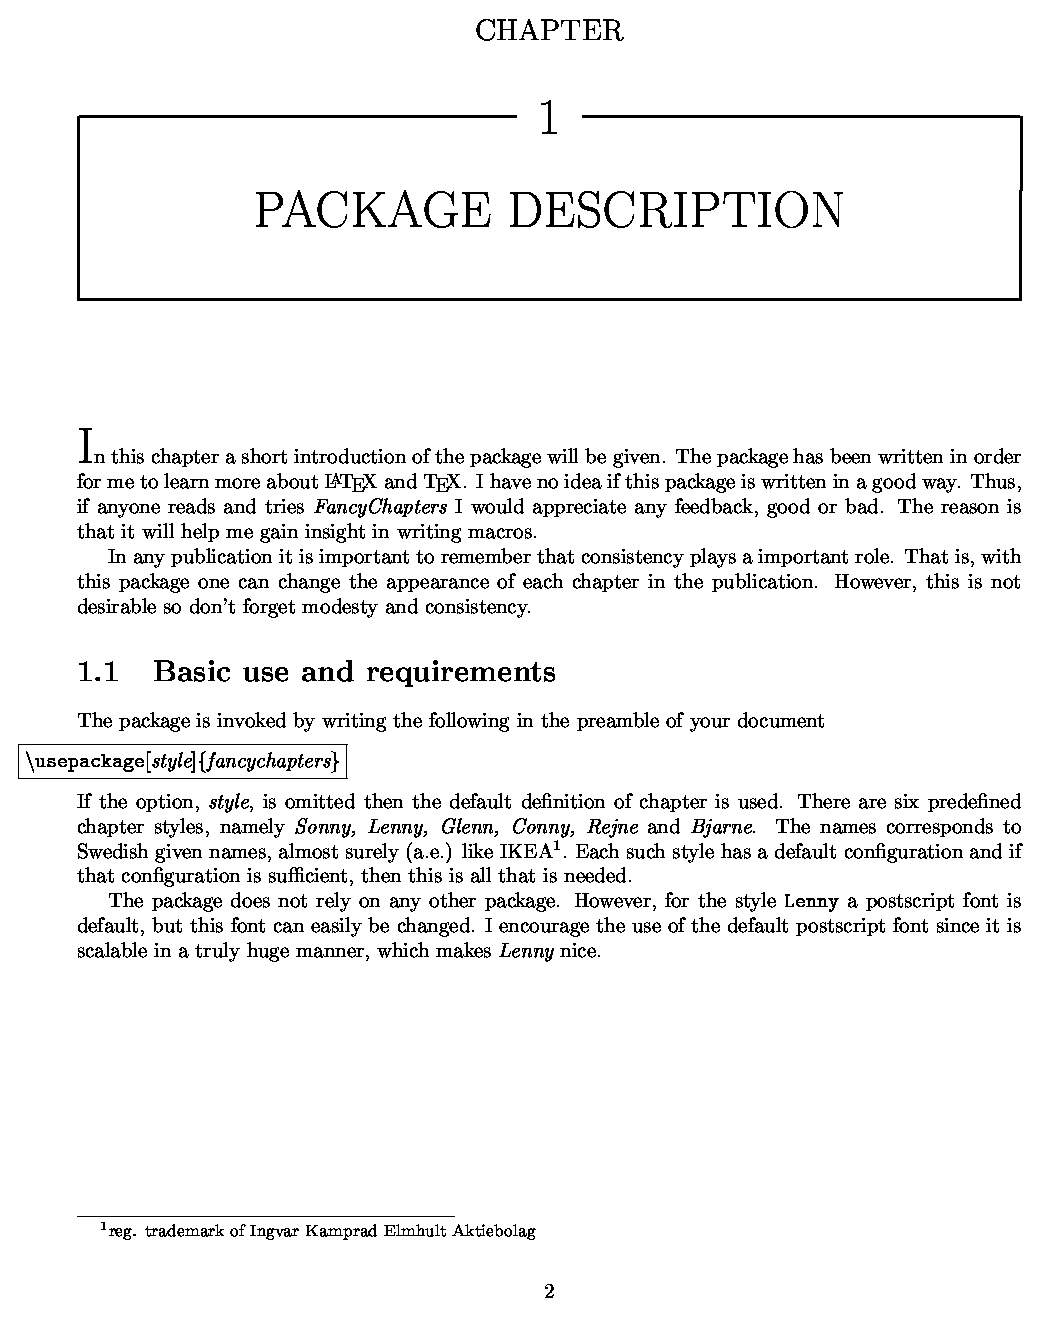
\includegraphics[height=6cm]{Rejne.eps}}
        \caption{The chapter style Rejne}
      \end{minipage}\hfill
    \end{figure}
    \section{The chapter Bjarne}
    The following settings have been used as default parameters
    {\small\begin{verbatim}
  \ChNameUpperCase \ChNameVar{\raggedleft\normalsize\rmfamily}
  \ChTitleUpperCase \ChTitleVar{\raggedleft\Large\rmfamily}
  \ChRuleWidth{1pt} \ChNumVar{\raggedleft\bfseries\Large}
     \end{verbatim}}
    \begin{figure}[h]
      \begin{minipage}{7 cm}
        \centerline{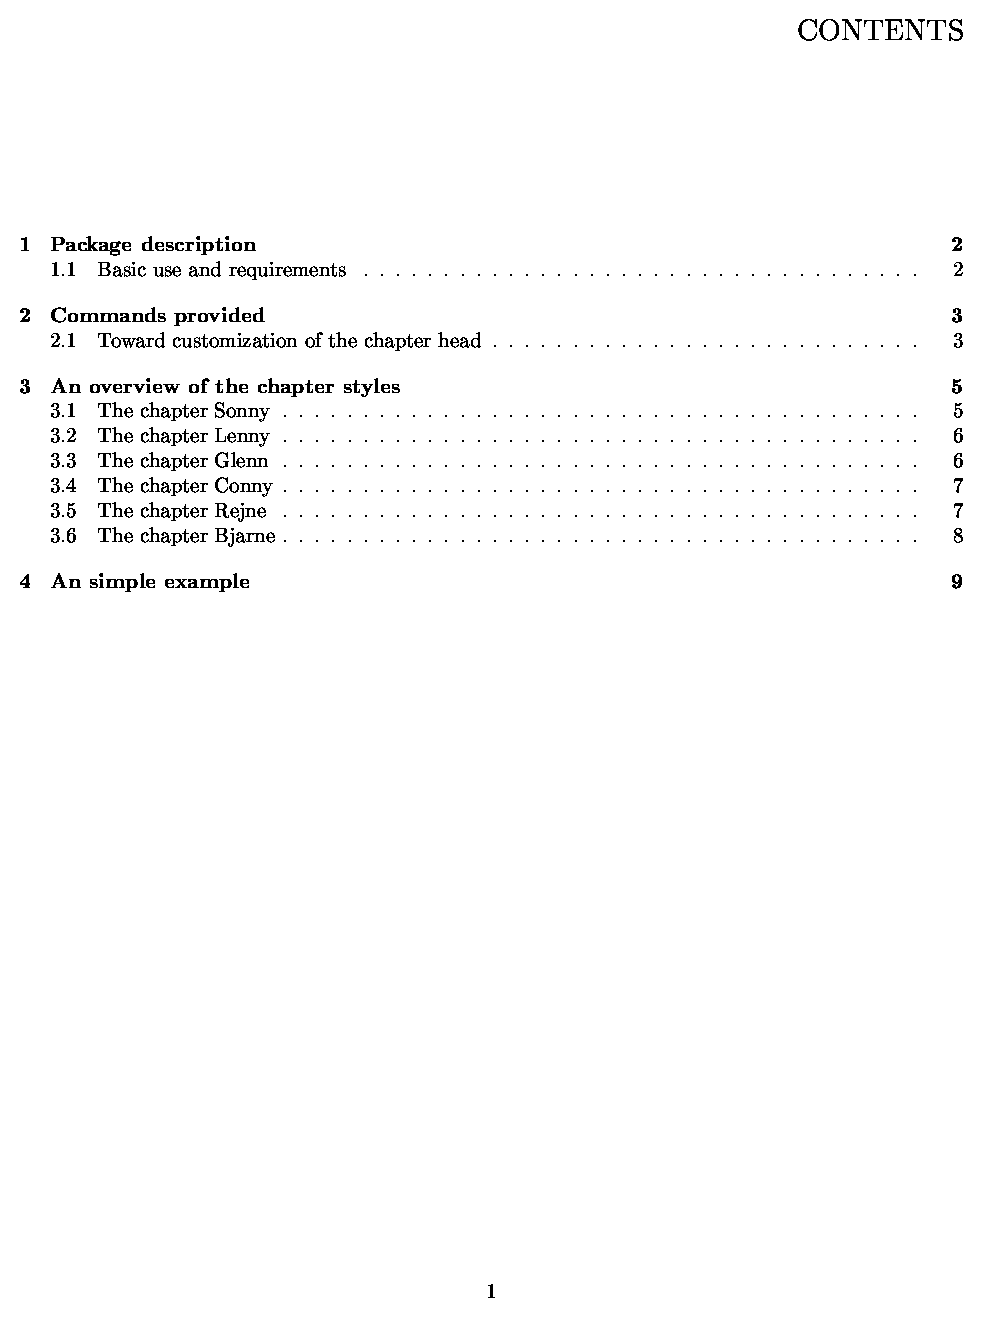
\includegraphics[height=6cm]{Bjarnes.eps}} 
        \caption{The stared chapter style Bjarne}
      \end{minipage}\hfill
      \begin{minipage}{7 cm}
        \centerline{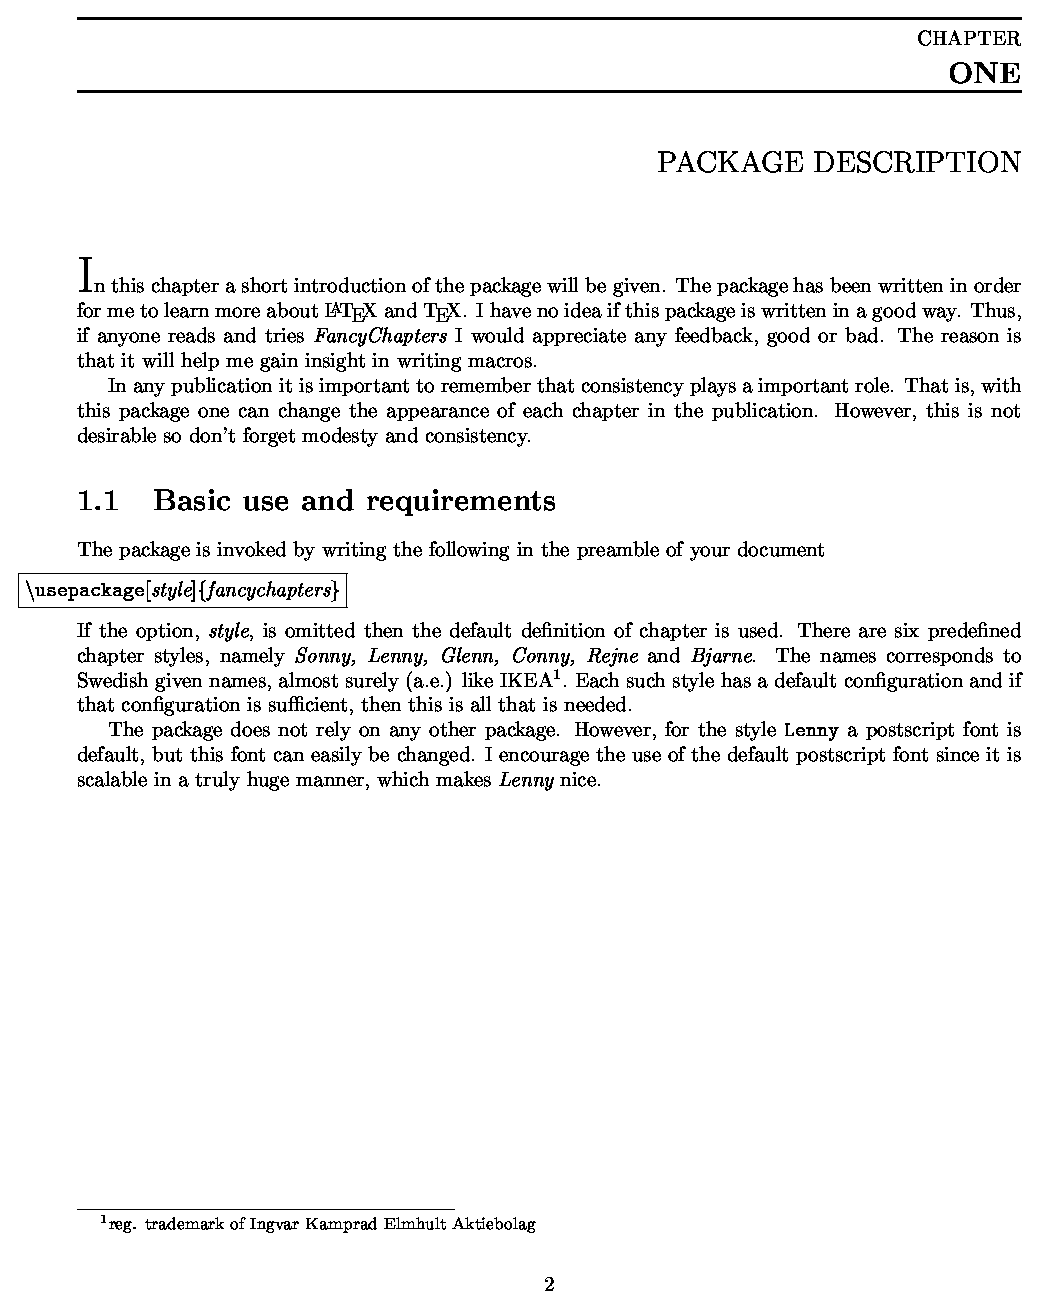
\includegraphics[height=6cm]{Bjarne.eps}}
        \caption{The chapter style Bjarne}
      \end{minipage}\hfill
    \end{figure}

    \section{The chapter Bjornstrup}
    The following settings have been used as default parameters
    {\small\begin{verbatim}
  \ChNumVar{\fontsize{76}{80}\usefont{OT1}{pzc}{m}{n}\selectfont}
  \ChTitleVar{\raggedleft\Large\sffamily\bfseries}
     \end{verbatim}}
    \begin{figure}[h]
      \begin{minipage}{7 cm}
        \centerline{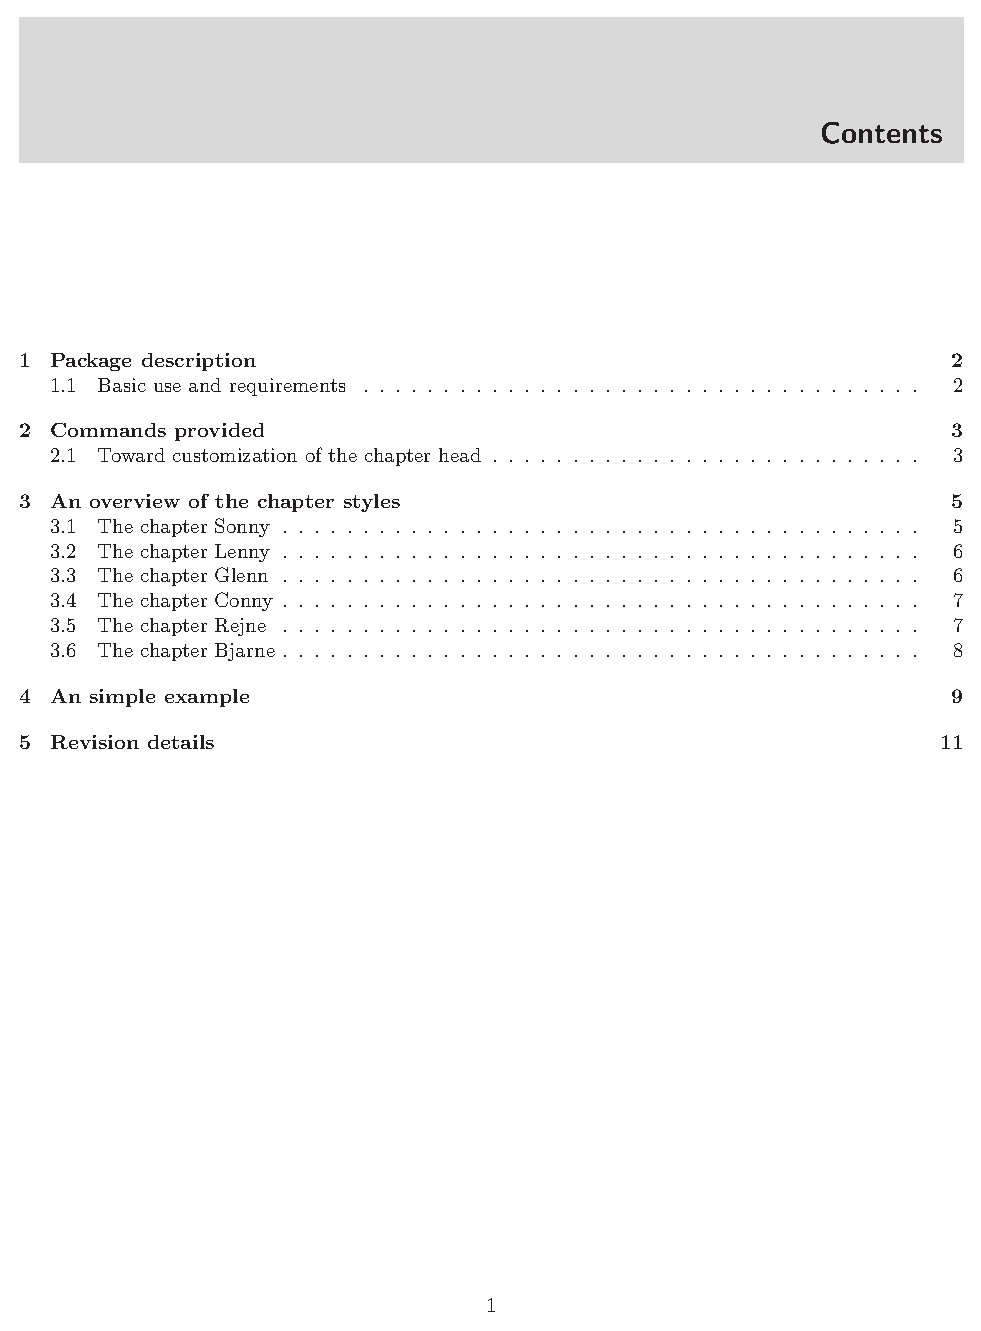
\includegraphics[height=6cm]{BjornstrupS.eps}} 
        \caption{The stared chapter style Bjornstrup}
      \end{minipage}\hfill
      \begin{minipage}{7 cm}
        \centerline{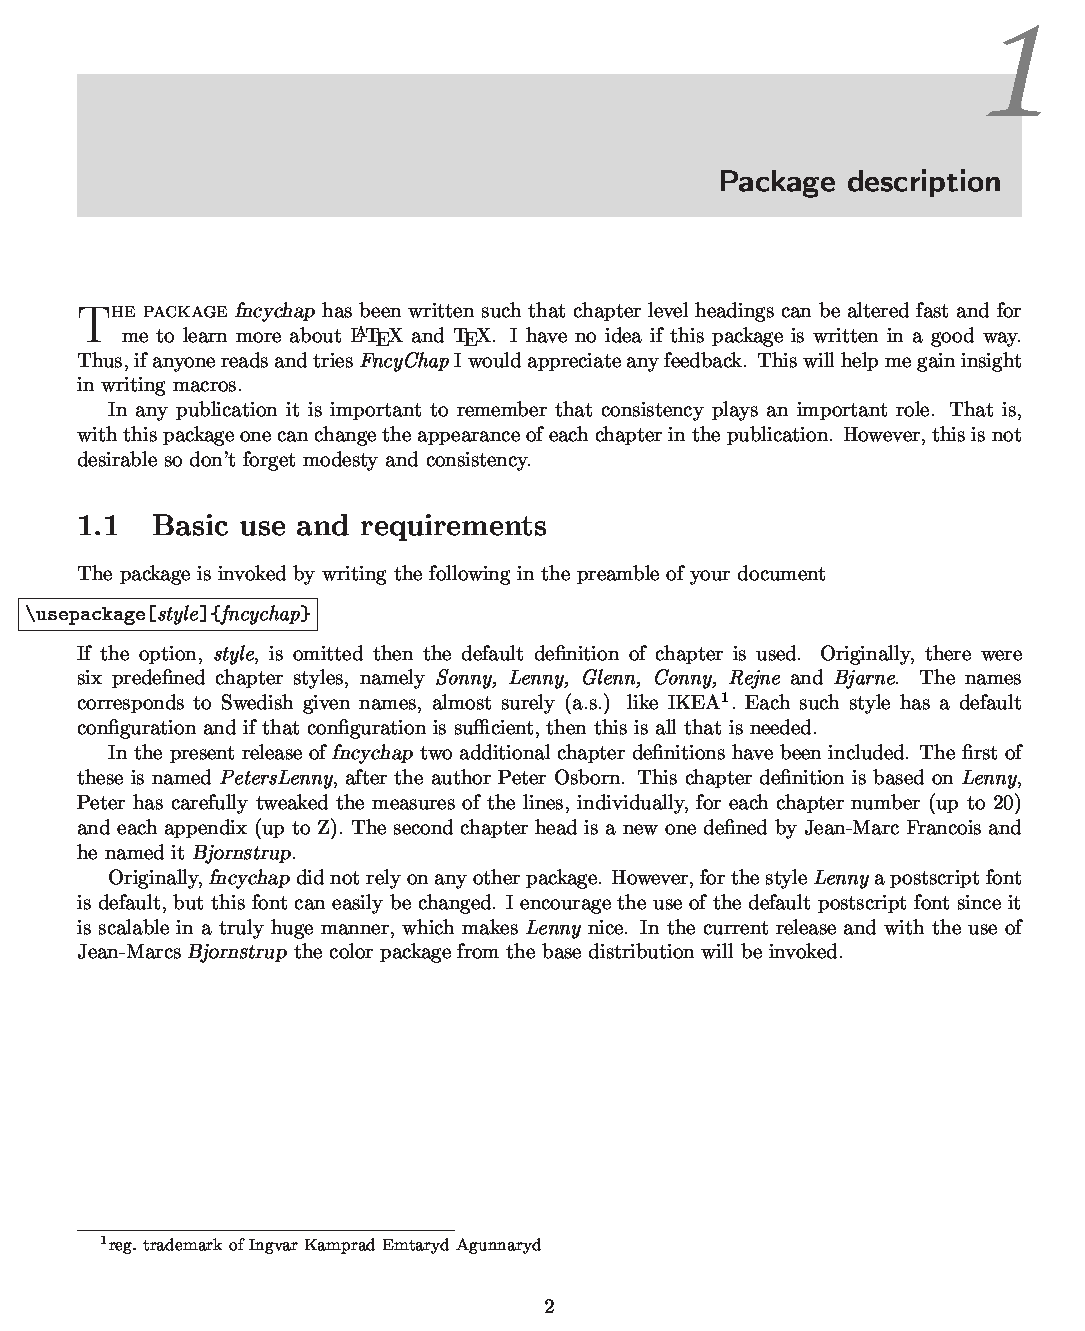
\includegraphics[height=6cm]{Bjornstrup.eps}}
        \caption{The chapter style Bjornstrup}
      \end{minipage}\hfill
    \end{figure}
\textbf{Note:} It appears as if the rendering in YAP (dvi previewer in
MikTeX) differs from dvips in that the gray box become
foreground. Thus, the chapter number is partly hidden. 
\enlargethispage{2cm}
  \chapter{A simple example}
    \lettrine{I}{f the pre-defined styles} do not fulfill your needs then you can
    modify the formating routines. The formatting is controlled by
    three commands. One might as well redefine the original
    chapter definitions using the \A{secdef} and \A{renewcommand}, see
    The \LaTeX{} companion. However, at the time of creating this
    package I decided that this was easier. The command\sk\\
    \nsp\fbox{\A{DOCH}}\sk\\
    formats the chapter name and number. The commands\sk\\
    \nsp\fbox{\A{DOTI}\{{\#1}\}}\sk\\
    and\sk\\
    \nsp\fbox{\A{DOTIS}\{{\#1}\}}\sk\\
    formats the chapter title for \A{chapter} and \A{chapter*} respectively.
    In order to modify these you will have to use the preamble along
    with the commands \A{makeatletter} and \A{makeatother}. The in
    addition some predefined parameters can be used. The predefined
    length variables are\sk\\
    \nsp\fbox{\A{mylen}, \A{myhi}, \A{px}, \A{py}, \A{pxx}, \A{pyy}
      and \A{RW}}\sk\\
    note that \A{RW} is special, since it is set by \A{ChRuleWidth}.
    The formatting controlled by \A{ChNameVar}, \A{ChNumVar} and
    \A{ChTitleVar} store their values in \A{CNV}, \A{CNoV} and \A{CTV}
    respectively. Finally, The functions \A{FmN}\{ \} and \A{FmTi}\{
    \} acts accordingly to \A{Ch***AsIs}, \A{Ch***UpperCase} and
    \A{Ch***LowerCase}. Note that the stars indicate appropriate
    substitution of text, see section~\ref{sec:TW}.

    To illustrate this lets define a new chapter style in which the
    Chapter name and number in a \A{fbox} and the chapter title
    centered. The \A{fboxrule} is linked to the predefined length
    \A{RW} so that it can be controlled by the command
    \A{ChRuleWidth}. Try this example at a computer near you.
    \begin{verbatim}
       \makeatletter
         \ChNameVar{\Large\rmfamily}    % sets the style for name
         \ChNumVar{\Huge}         % sets the style for digit
         \ChTitleVar{\Large\rmfamily\centering}   % sets the style for title
         \ChRuleWidth{4pt}        % Set RW=4pt
         \ChNameUpperCase         % Make name uppercase
         \renewcommand{\DOCH}{%
           \setlength{\fboxrule}{\RW} % Let fbox lines be controlled by
                                      % \ChRuleWidth

           \fbox{\CNV\FmN{\@chapapp}\space \CNoV\thechapter}\par\nobreak
           \vskip 40\p@}

         \renewcommand{\DOTI}[1]{%
           \CTV\FmTi{#1}\par\nobreak
           \vskip 40\p@}
         \renewcommand{\DOTIS}[1]{%
           \CTV\FmTi{#1}\par\nobreak
           \vskip 40\p@}
       \makeatother
    \end{verbatim}
    That is all there is to it. Note that the commands \A{DOTI} and
    \A{DOTIS} can be redefined anywhere in the document, but that is
    not a good idea. Suppose that you want to use the
    \A{TheAlphaChapter}. This can be done by initially chose the style
    {\em Bjarne}\/ and then redefine \A{DOCH}, \A{DOTI} and \A{DOTIS}.
    \chapter{Revision details}
     \lettrine{T}{his is version 1.34}, some minor problems have been
     addressed and two new predefined chapter heads have been
     incorporated. The upper case and lower case handling have been
     corrected. A bad behavior in changes between \verb+\frontmatter+,
     \verb+\mainmatter+ and  \verb+\backmatter+, have been fixed.   

     In version 1.33 Rejne definition streched text caused ugly gaps
     in the vrule aligned with the title text. A compatibility problem
     with the KOMA class 'scrbook.cls' the remedy is a redefinition of
     '\@schapter' in line with that used in KOMA. This might not be
     good since it differs from the base definition. A spell error was
     corrected.
 
      In version 1.3, a problem with appendices in the Bjarne style was
      corrected. Wrong behavior, for the commands
      \verb+\frontmatter+, \verb+\mainmatter+ and  \verb+\backmatter+
      was dealt with. 

      In the release 1.11 of the current package. A bug
      fix of the Lenny option was included. The problem, reported
      by Diab Jerius, occurred (underfull vbox) when the option Lenny
      was used in conjunction with \A{section}-command such that the
      section is typeset at the next page. This caused one line to be
      misplaced. The remedy was to box the chapter title.

      In the release (1.1) of the current package. A
      modification was made such that it will work with the book
      class. The problem occurred when the fncychap styles Conny,
      Rejne, Bjarne or Glenn were used in conjunction with the
      \LaTeX{} command \A{tabelofcontents}. The exact reason for the
      error is not yet found. The problem was reported by Olivier Guibe.

      In the prior release there were no major improvements of the
      package. However, the package name was changed in order to
      conform with the (DOS) requirement of eight characters. I also
      received some feedback, informing me that the \LaTeX{} base have
      to be post 1994/12/01.  This information has been included in
      the package such that if an old base is used a warning will be
      written into the {\tt
        log}.

      \section*{Release history:}
      \begin{description}
        \item[Release 1] 1996/12/13 FancyChapters 1.0b
        \item[Release 2] 1997/01/08 FncyChap 1.0 (Name change, base
          date option)
        \item[Release 3] 1997/01/22 FncyChap 1.1 (Bug fix)
        \item[Release 4] 1997/04/06 FncyChap 1.11 (Bug fix)
        \item[Release 5] 2004/09/20 FncyChap 1.3 (Bug fix)
        \item[Release 6] 2005/08/09 FncyChap 1.33 (Bug fix)
        \item[Release 7] 2007/07/31 FncyChap 1.34 (Bug fix)
      \end{description}

\end{document}
%%% Local Variables: 
%%% mode: latex
%%% TeX-master: t
%%% End: 














